\chapter{Introduction}
\label{chp:introduction} 
\section{\label{sec:motivation}Motivation}
With the increasing focus on power consumption and small design-size, hardware manufacturer are forced to develop their products with these parameters in mind. Architectural exploration of hardware plays a vital role in the process of creating integrated circuits with the best trade-offs between speed, area, and power consumption for a given specification. The process of architectural exploration is a tedious and time-consuming process, involving many steps. During the exploration, a number of hardware architectures are built and evaluated based on minimum performance requirements and worst-case operational scenarios. By generating a large number of designs with great diversity, a satisfactory result can be achieved. The number of architectures that can be evaluated is limited by time and resources. \gls{hls} is a compelling alternative to shorten this process. By reducing the time for creating each potential design, the number of evaluated designs can be increased, with the potential of generating far more diversity between the architectures than what would ever have been possible by parameterized RTL.

Figure \ref{fig:motivationflow} shows a typical design process for an \gls{dsp} application on the left side, and the reduced flow using a \gls{hls}-based framework on the right side. It is easy to see that the effort the designer has to put into the process is drastically reduced with the second alternative.

\begin{figure}[hbpt]
\centering
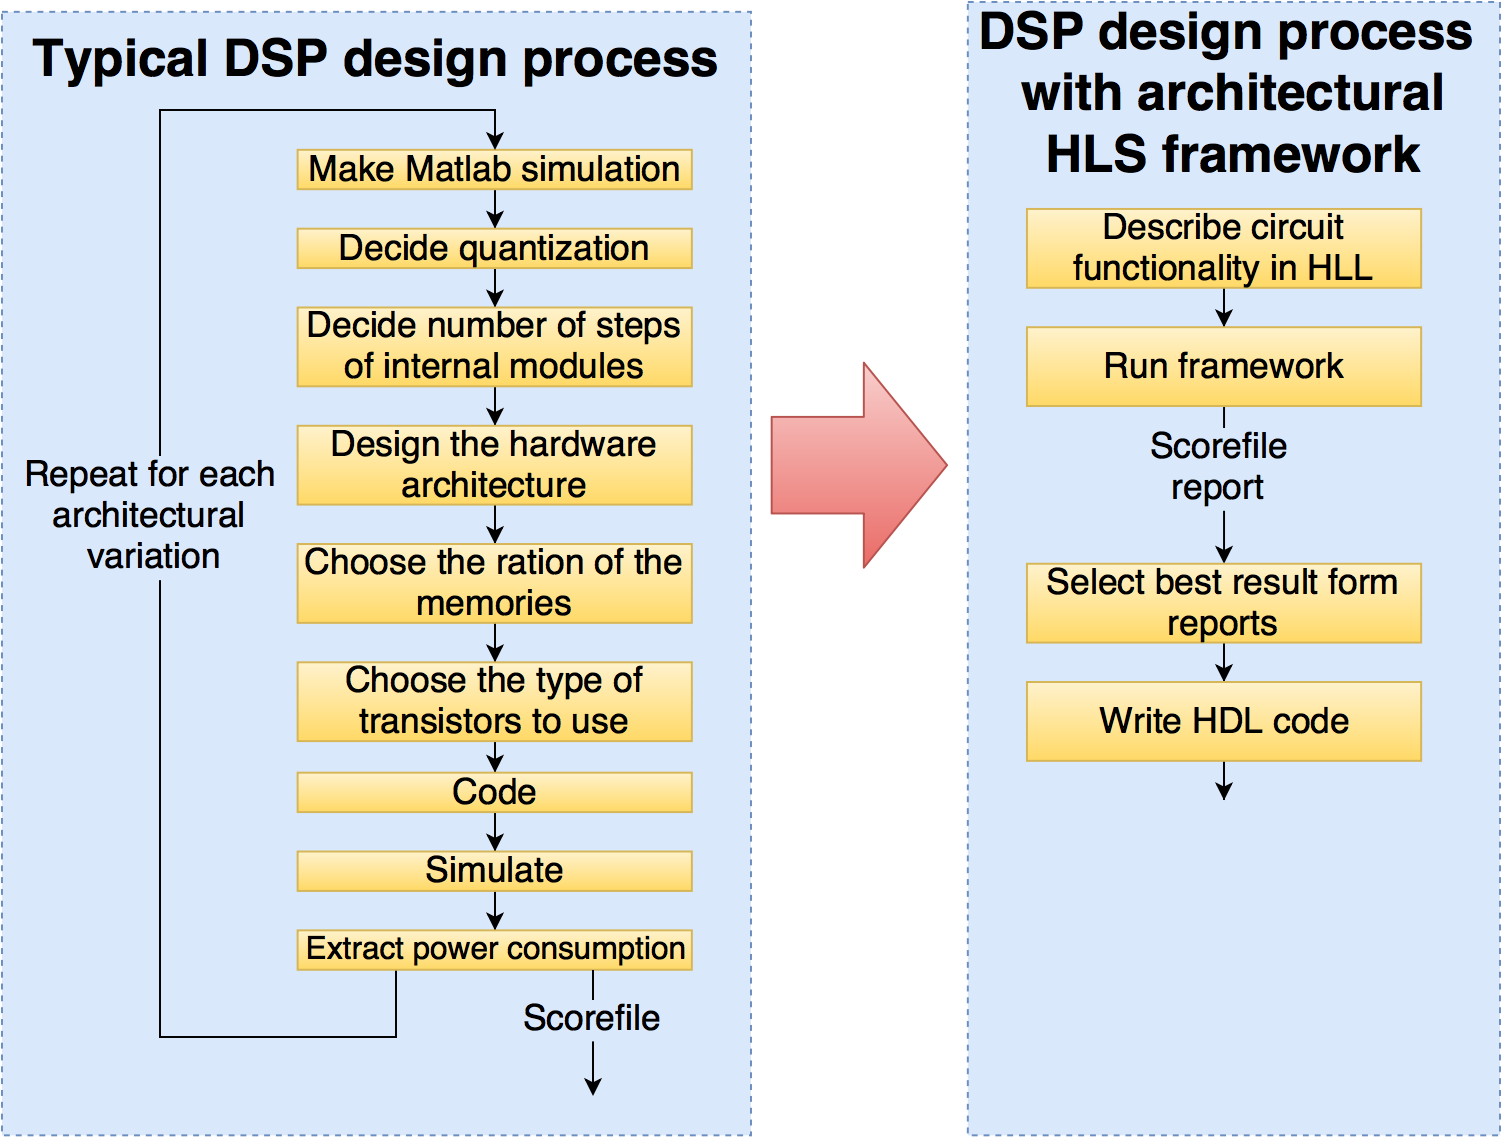
\includegraphics[width=0.75\textwidth]{../figs/Motivation.png}
\caption{\label{fig:motivationflow}Typical work-flow of a DSP design process compared to workflow using HLS framework.}
\end{figure}

\section{Previous work}
In my specialization project \cite{holm2015pro}, conducted during the autumn of 2015, I investigated the academic, open source tool LegUp. LegUp provides ANSI-C to Verilog high-level synthesis, but their focus is targeted towards implementation on FPGAs. The official target support of the output is limited to a few boards from the FPGA manufacturer Altera, and beta-support for a single board from Xilinx. The desired ultimate goal of a framework for architectural exploration will target ASIC implementations. The findings from the specialization project were that there are some fundamental issues with using LegUp, in its current form, limiting its usability for such a framework. The issues are mainly related to input and output of the generated modules, structure of memory management, and size of signals. A framework for architectural exploration of hardware, using \gls{hls}, were proposed in \cite{holm2015pro}. An illustrration showing the tool- and information-flow of the framework is shown in \cref{fig:frameworkflow}.

\begin{figure}[hbpt]
\centering
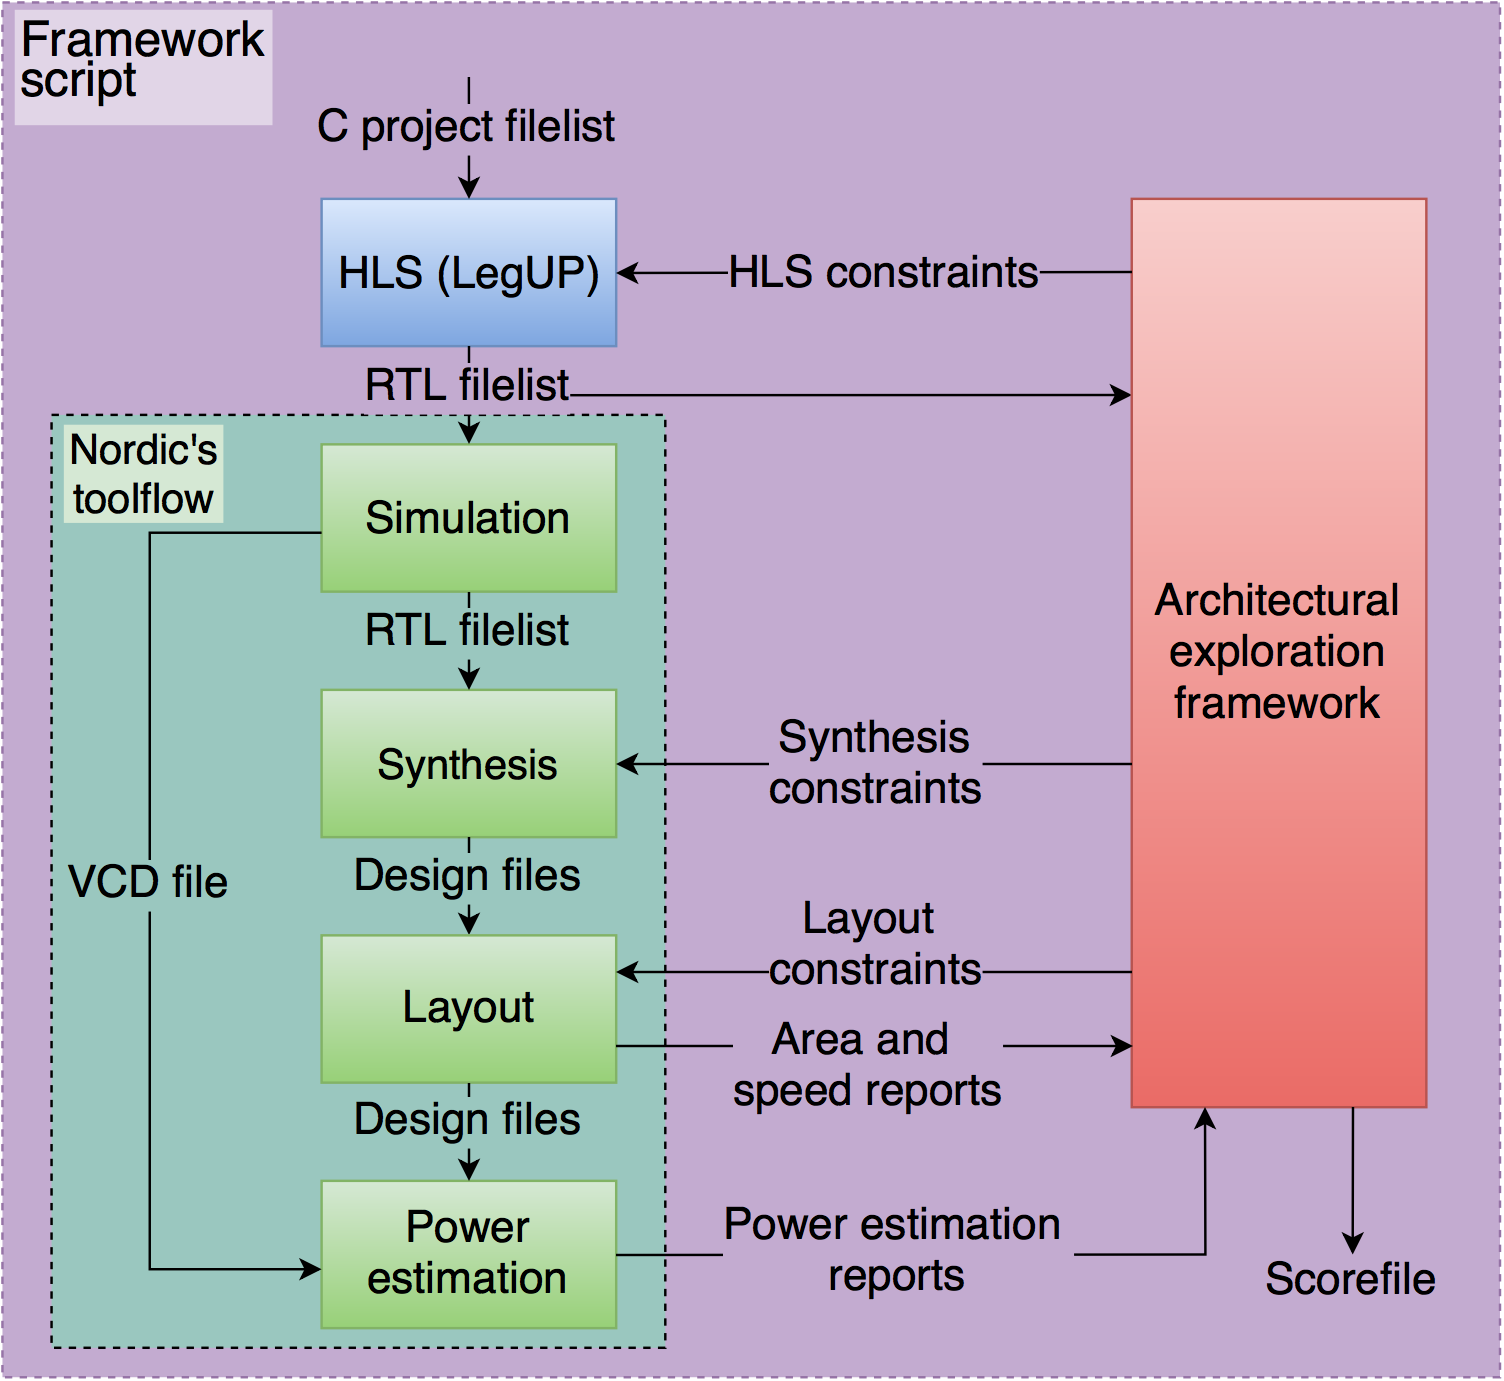
\includegraphics[width=0.75\textwidth]{../figs/Framework.png}
\caption{\label{fig:frameworkflow}Proposed framework-solution \cite{holm2015pro}.}
\end{figure}

\section{\label{sec:projectobj}Project objectives}
The initial goals of the specialization project were found to be a bit exaggerated. For this Master thesis it were decided to focus on a smaller part of the ultimate goal, to get the necessary basics working good before proceeding with the rest. The goal of this Master thesis is therefore first to resolve the issues encountered during the specialization project. At the start of the project period, it were not certain if all issues were resolvable, or how time consuming it would be. A prioritized list of objectives were therefore created.

\newcommand\litem[1]{\item{\bfseries #1\\}}
\begin{enumerate}
\litem{Explore approaches} Two approaches to resolve the issued were described in \cite{holm2015pro}. The first step of this thesis will be to explore both these alternatives and look at positives and negatives with each method. The outcome of this objective will affect the rest of the work with this thesis, making it an important decision. All aspects of the two approaches must therefore be taken into consideration before making a choice.
\litem{Resolve issues} For LegUp to be usable in a framework for architectural exploration, it is vital that tool is adapted to generated Verilog suitable for ASIC implementation. This objective is thought to be the most time-consuming, and its outcome is very uncertain. However, if completed successfully, the use-space of LegUp can be extended to other concepts. LegUp’s architecture is, like the input language C, quite memory-bound. RAMs, memory controllers, and pointers are used for many things where a simple signal could have given the same result. It should be looked into if this memory-architecture can be changed by de-referencing pointers or turn memory elements into generic signals. A proper way of handling inputs and outputs should also be implemented, to avoid being limited to a certain amount of ports on the generated designs.
\litem{Create framework} When the issues has been resolved, the work with creating a framework for architectural exploration can be started. The framework will be based on the figure shown in \cref{fig:frameworkflow}, using various scripts and program to run the tool-flow, generating constraints and create scorefiles. The framework should be easy to use and ideally be able to execute without any interactions with the user.
\litem{Proof-of-concept} To verify and illustrate the concept in action, a proof-of-concept will be created. By creating one or more reference designs that will be run through the framework, it is expected to get a wide variety of generated designs with varying results in terms of area, power consumption, and speed. The reference design will also be implemented directly in Verilog \gls{hdl}, to compare and calculate the overhead of the \gls{hls}-generated designs.
\litem{Evaluation} Based on the results from the conducted proof-of-concept, a re-evaluate of LegUp's usefulness in a framework for architectural exploration of digital hardware. This evaluation will be based on the deviation of the results among the generated designs, as well as the overhead compared to the design written in Verilog. Other aspects can be considered, like how well the adaption of LegUp is performed and how well the generated Verilog \gls{hdl} synthesize for ASIC architectures.
\litem{Techniques for reducing overhead} The typical overhead of \gls{hls}-tools are in the range of 30-40\%. One of the initial objectives of this concept included the integration of  Nordic Semiconductor's coding style and practices, the \gls{ddvc} \cite{nordicddvc}, into LegUp's Verilog libraries. This include things like interfaces, parameters, naming conventions, power/clock domains, etc. It is assumed that this can give a large reduction of the overhead generated by the \gls{hls}-tool, when integrated into Nordic Semiconductor's existing modules.
\end{enumerate}

\section{Overview of the thesis}
In general, this thesis is divided into chapters, each presenting one of the projecet objectives discribed above. In \cref{chp:background}, the background and theory required to understand the rest of the thesis is described. Point one and two from the project objectives list given above is described in \cref{chp:adaptinglegup}. Chapter \ref{chp:toolflowex} presents a thorough description of the tool-flow in LegUp and in the framework, using an example design. In \cref{chp:createframework} the third objective, the process of creating a framework, is described. The fourth objective, to create a proof-of-concept, is presented in \cref{chp:frameworkresults}. The evaluation of the proof-of-concept results, corresponding to the fifth objective, as well as a discussion of LegUp in general, with focus on its usefulness in the created framework, has been presented in \cref{chp:discussion}. Finally the work is summarized and concluded in \cref{chp:conclusion}.
